\documentclass[11pt,a4paper,]{article}
\usepackage{lmodern}

\usepackage{amssymb,amsmath}
\usepackage{ifxetex,ifluatex}
\usepackage{fixltx2e} % provides \textsubscript
\ifnum 0\ifxetex 1\fi\ifluatex 1\fi=0 % if pdftex
  \usepackage[T1]{fontenc}
  \usepackage[utf8]{inputenc}
\else % if luatex or xelatex
  \usepackage{unicode-math}
  \defaultfontfeatures{Ligatures=TeX,Scale=MatchLowercase}
\fi
% use upquote if available, for straight quotes in verbatim environments
\IfFileExists{upquote.sty}{\usepackage{upquote}}{}
% use microtype if available
\IfFileExists{microtype.sty}{%
\usepackage[]{microtype}
\UseMicrotypeSet[protrusion]{basicmath} % disable protrusion for tt fonts
}{}
\PassOptionsToPackage{hyphens}{url} % url is loaded by hyperref
\usepackage[unicode=true]{hyperref}
\hypersetup{
            pdftitle={Peeking inside FFORMS: Feature-based FORecast Model Selection},
            pdfkeywords={forecasting, time series, machine learning interpretability, black-box
models, LIME},
            pdfborder={0 0 0},
            breaklinks=true}
\urlstyle{same}  % don't use monospace font for urls
\usepackage{geometry}
\geometry{left=2.5cm,right=2.5cm,top=2.5cm,bottom=2.5cm}
\usepackage[style=authoryear-comp,]{biblatex}
\addbibresource{references.bib}
\usepackage{longtable,booktabs}
% Fix footnotes in tables (requires footnote package)
\IfFileExists{footnote.sty}{\usepackage{footnote}\makesavenoteenv{long table}}{}
\usepackage{graphicx,grffile}
\makeatletter
\def\maxwidth{\ifdim\Gin@nat@width>\linewidth\linewidth\else\Gin@nat@width\fi}
\def\maxheight{\ifdim\Gin@nat@height>\textheight\textheight\else\Gin@nat@height\fi}
\makeatother
% Scale images if necessary, so that they will not overflow the page
% margins by default, and it is still possible to overwrite the defaults
% using explicit options in \includegraphics[width, height, ...]{}
\setkeys{Gin}{width=\maxwidth,height=\maxheight,keepaspectratio}
\IfFileExists{parskip.sty}{%
\usepackage{parskip}
}{% else
\setlength{\parindent}{0pt}
\setlength{\parskip}{6pt plus 2pt minus 1pt}
}
\setlength{\emergencystretch}{3em}  % prevent overfull lines
\providecommand{\tightlist}{%
  \setlength{\itemsep}{0pt}\setlength{\parskip}{0pt}}
\setcounter{secnumdepth}{5}

% set default figure placement to htbp
\makeatletter
\def\fps@figure{htbp}
\makeatother


\title{Peeking inside FFORMS: Feature-based FORecast Model Selection}

%% MONASH STUFF

%% CAPTIONS
\RequirePackage{caption}
\DeclareCaptionStyle{italic}[justification=centering]
 {labelfont={bf},textfont={it},labelsep=colon}
\captionsetup[figure]{style=italic,format=hang,singlelinecheck=true}
\captionsetup[table]{style=italic,format=hang,singlelinecheck=true}

%% FONT
\RequirePackage{bera}
\RequirePackage{mathpazo}

%% HEADERS AND FOOTERS
\RequirePackage{fancyhdr}
\pagestyle{fancy}
\rfoot{\Large\sffamily\raisebox{-0.1cm}{\textbf{\thepage}}}
\makeatletter
\lhead{\textsf{\expandafter{\@title}}}
\makeatother
\rhead{}
\cfoot{}
\setlength{\headheight}{15pt}
\renewcommand{\headrulewidth}{0.4pt}
\renewcommand{\footrulewidth}{0.4pt}
\fancypagestyle{plain}{%
\fancyhf{} % clear all header and footer fields
\fancyfoot[C]{\sffamily\thepage} % except the center
\renewcommand{\headrulewidth}{0pt}
\renewcommand{\footrulewidth}{0pt}}

%% MATHS
\RequirePackage{bm,amsmath}
\allowdisplaybreaks

%% GRAPHICS
\RequirePackage{graphicx}
\setcounter{topnumber}{2}
\setcounter{bottomnumber}{2}
\setcounter{totalnumber}{4}
\renewcommand{\topfraction}{0.85}
\renewcommand{\bottomfraction}{0.85}
\renewcommand{\textfraction}{0.15}
\renewcommand{\floatpagefraction}{0.8}

%\RequirePackage[section]{placeins}

%% SECTION TITLES
\RequirePackage[compact,sf,bf]{titlesec}
\titleformat{\section}[block]
  {\fontsize{15}{17}\bfseries\sffamily}
  {\thesection}
  {0.4em}{}
\titleformat{\subsection}[block]
  {\fontsize{12}{14}\bfseries\sffamily}
  {\thesubsection}
  {0.4em}{}
\titlespacing{\section}{0pt}{*5}{*1}
\titlespacing{\subsection}{0pt}{*2}{*0.2}


%% TITLE PAGE
\def\Date{\number\day}
\def\Month{\ifcase\month\or
 January\or February\or March\or April\or May\or June\or
 July\or August\or September\or October\or November\or December\fi}
\def\Year{\number\year}

\makeatletter
\def\wp#1{\gdef\@wp{#1}}\def\@wp{??/??}
\def\jel#1{\gdef\@jel{#1}}\def\@jel{??}
\def\showjel{{\large\textsf{\textbf{JEL classification:}}~\@jel}}
\def\nojel{\def\showjel{}}
\def\addresses#1{\gdef\@addresses{#1}}\def\@addresses{??}
\def\cover{{\sffamily\setcounter{page}{0}
        \thispagestyle{empty}%
        \vspace*{-2cm}
        \centerline{\raisebox{-1.8cm}{\includegraphics[width=5cm]{MBSportrait}}\hspace*{9cm} ISSN 1440-771X}\vspace{0.99cm}
        \begin{center}\Large
        Department of Econometrics and Business Statistics\\[.5cm]
        \scriptsize http://business.monash.edu/econometrics-and-business-statistics/research/publications
        \end{center}\vspace{2cm}
        \begin{center}
        \fbox{\parbox{14cm}{\begin{onehalfspace}\centering\Huge\vspace*{0.3cm}
                \textsf{\textbf{\expandafter{\@title}}}\vspace{1cm}\par
                \LARGE\@author\end{onehalfspace}
        }}
        \end{center}
        \vfill
                \begin{center}\Large
                \Month~\Year\\[1cm]
                Working Paper \@wp
        \end{center}}}
\def\pageone{{\sffamily\setstretch{1}%
        \thispagestyle{empty}%
        \vbox to \textheight{%
        \raggedright\baselineskip=1.2cm
     {\fontsize{24.88}{30}\sffamily\textbf{\expandafter{\@title}}}
        \vspace{2cm}\par
        \hspace{1cm}\parbox{14cm}{\sffamily\large\@addresses}\vspace{1cm}\vfill
        \hspace{1cm}{\large\Date~\Month~\Year}\\[1cm]
        \hspace{1cm}\showjel\vss}}}
\def\blindtitle{{\sffamily
     \thispagestyle{plain}\raggedright\baselineskip=1.2cm
     {\fontsize{24.88}{30}\sffamily\textbf{\expandafter{\@title}}}\vspace{1cm}\par
        }}
\def\titlepage{{\cover\newpage\pageone\newpage\blindtitle}}

\def\blind{\def\titlepage{{\blindtitle}}\let\maketitle\blindtitle}
\def\titlepageonly{\def\titlepage{{\pageone\end{document}}}}
\def\nocover{\def\titlepage{{\pageone\newpage\blindtitle}}\let\maketitle\titlepage}
\let\maketitle\titlepage
\makeatother

%% SPACING
\RequirePackage{setspace}
\spacing{1.5}

%% LINE AND PAGE BREAKING
\sloppy
\clubpenalty = 10000
\widowpenalty = 10000
\brokenpenalty = 10000
\RequirePackage{microtype}

%% PARAGRAPH BREAKS
\setlength{\parskip}{1.4ex}
\setlength{\parindent}{0em}

%% HYPERLINKS
\RequirePackage{xcolor} % Needed for links
\definecolor{darkblue}{rgb}{0,0,.6}
\RequirePackage{url}

\makeatletter
\@ifpackageloaded{hyperref}{}{\RequirePackage{hyperref}}
\makeatother
\hypersetup{
     citecolor=0 0 0,
     breaklinks=true,
     bookmarksopen=true,
     bookmarksnumbered=true,
     linkcolor=darkblue,
     urlcolor=blue,
     citecolor=darkblue,
     colorlinks=true}

%% KEYWORDS
\newenvironment{keywords}{\par\vspace{0.5cm}\noindent{\sffamily\textbf{Keywords:}}}{\vspace{0.25cm}\par\hrule\vspace{0.5cm}\par}

%% ABSTRACT
\renewenvironment{abstract}{\begin{minipage}{\textwidth}\parskip=1.4ex\noindent
\hrule\vspace{0.1cm}\par{\sffamily\textbf{\abstractname}}\newline}
  {\end{minipage}}


\usepackage[T1]{fontenc}
\usepackage[utf8]{inputenc}

\usepackage[showonlyrefs]{mathtools}
\usepackage[no-weekday]{eukdate}

%% BIBLIOGRAPHY

\makeatletter
\@ifpackageloaded{biblatex}{}{\usepackage[style=authoryear-comp, backend=biber, natbib=true]{biblatex}}
\makeatother
\ExecuteBibliographyOptions{bibencoding=utf8,minnames=1,maxnames=3, maxbibnames=99,dashed=false,terseinits=true,giveninits=true,uniquename=false,uniquelist=false,doi=false, isbn=false,url=true,sortcites=false}

\DeclareFieldFormat{url}{\texttt{\url{#1}}}
\DeclareFieldFormat[article]{pages}{#1}
\DeclareFieldFormat[inproceedings]{pages}{\lowercase{pp.}#1}
\DeclareFieldFormat[incollection]{pages}{\lowercase{pp.}#1}
\DeclareFieldFormat[article]{volume}{\mkbibbold{#1}}
\DeclareFieldFormat[article]{number}{\mkbibparens{#1}}
\DeclareFieldFormat[article]{title}{\MakeCapital{#1}}
\DeclareFieldFormat[inproceedings]{title}{#1}
\DeclareFieldFormat{shorthandwidth}{#1}
% No dot before number of articles
\usepackage{xpatch}
\xpatchbibmacro{volume+number+eid}{\setunit*{\adddot}}{}{}{}
% Remove In: for an article.
\renewbibmacro{in:}{%
  \ifentrytype{article}{}{%
  \printtext{\bibstring{in}\intitlepunct}}}

\makeatletter
\DeclareDelimFormat[cbx@textcite]{nameyeardelim}{\addspace}
\makeatother
\renewcommand*{\finalnamedelim}{%
  %\ifnumgreater{\value{liststop}}{2}{\finalandcomma}{}% there really should be no funny Oxford comma business here
  \addspace\&\space}


\wp{no/yr}
\jel{C10,C14,C22}


\blind



\date{\sf\Date~\Month~\Year}
\makeatletter
 \lfoot{\sf\@date}
\makeatother

%% Any special functions or other packages can be loaded here.
%% Any special functions or other packages can be loaded here.
\usepackage{tikz}
\usepackage{algorithm}
\usepackage{algpseudocode}
\usepackage{amsthm}
\usepackage{amsmath,bm}
\usepackage{paralist}
\usepackage{todonotes}
\usepackage{ctable}
\usepackage{multirow}
\usepackage{lscape}
\usepackage{rotating}
\usepackage{float} 
\floatplacement{figure}{H} 

\def\sectionautorefname{Section}
\captionsetup[figure]{font=small}
\captionsetup[table]{font=small}
\def\var{\text{Var}}
\allowdisplaybreaks
\sloppy

%% LINE AND PAGE BREAKING
\clubpenalty = 4500
\widowpenalty = 4500
\brokenpenalty = 4500


\def\yes{$\checkmark$}

\setlength{\abovedisplayskip}{5pt}
\setlength{\belowdisplayskip}{5pt}
\setlength{\abovedisplayshortskip}{0pt}
\setlength{\belowdisplayshortskip}{0pt}


\begin{document}
\maketitle
\begin{abstract}
Features of time series are considered to be an important factor in
identifying suitable forecast-models. \textcite{fforms} proposed a
classification framework, called FFORMS (Feature-based FORecast Model
Selection), which selects forecast models based on features calculated
from the time series. FFORMS framework builds a mapping that relates the
features of time series to the ``best'' forecast-model using the random
forest algorithm. In this paper we make an effort to explore what is
happening under the hood of FFORMS framework and thereby gain an
understanding of what features led to the different choices of
forecast-models and how different features influence the predicted
outcome. This is accomplished by using model-agnostic machine learning
interpretability approaches. Partial-dependency plots are used to
visualize both main and interaction effects of features. The results of
this study provide a valuable insight into how different features and
their interactions affect the choice of forecast-model selection. This
gives a more refine picture of the relationship between features and the
choice of forecast-model which is particularly valuable for ongoing
research in the field of feature-based time series analysis.
\end{abstract}
\begin{keywords}
forecasting, time series, machine learning interpretability, black-box
models, LIME
\end{keywords}

\section{Introduction}\label{intro}

The time series forecasting field has been evolving for a long time and
has introduced a wide variety of forecasting methods. However, for a
given time series the selection of an appropriate forecast-models among
many possibilities is not straight forward. This selection is one of the
most difficult tasks as each method perform best for some but not all
tasks. The features of time series are considered to be an important
factor in identifying suitable forecasting models
\autocites{collopy1992rule}{meade2000evidence}{makridakis2000m3}{wang2009rule}.
However, a comprehensive description of relationship between the
features and the performance of algorithms is rarely discussed in the
field of forecasting.

There have been several recent studies on the use of meta-learning
approaches to automate the forecast model selection based on the
features computed from the time series
\autocites{shah1997model}{prudencio2004meta}{lemke2010meta}{kuck2016meta}.
Meta-learning approach provides a systematic guidance on model selection
based on knowledge acquire from historical data set. The key idea is,
forecast-model selection is posed as a supervised learning task. Each
time series in the meta-data set is represented as a vector of features
and labelled according to the ``best'' forecast-model (i.e.~lowest MASE,
etc.). Then a meta-learner is trained to identify suitable
forecast-model (usually a machine learning algorithm is used). With the
era of big data, such an automated model selection process is necessary
because the cost of invoking all possible forecas-models is prohibitive.
However, these work suffer from the limitation of providing answers to
the questions of: i) How features are related to the property being
modelled?; ii) How features interact with each other to identify the
suitable forecasting method?; and iii) Which features contribute the
most to classification process?, that can enhance the understanding of
relations between features and model outcomes. To the best of our
knowledge, very limited efforts have been taken to understand how the
models are making its decisions and what is really happening inside
these complex model structures. Understanding the role of features is
worthwhile even if producing an accurate predictions is the only
objective of the modelling. This is because the less transparency of the
model may be distrusted regardless of their predictive performance.

On the other hand, aside from the goal of developing automated
forecast-model selection framework few researchers have made an attempt
to provide a description of relationship between the features and the
performance of algorithms
\autocites{schnaars1984situational}{wang2009rule}{lemke2010meta}{petropoulos2014horses}.
However, these studies are limited by the scale of problem instances
used, diversity of forecasting-methods used, limited number of features
considered, and modelling approached used to identify the relationship
between features and forecast model performance. Most of these studies
are typically restricted to simple statistical techniques such as simple
linear models, decision trees, cluster analysis, etc.

To fill this gap, this paper makes a first step towards providing a
comprehensive explanation of the relationship between time series
features and forecast-model selection using machine learning
interpretability techniques. This paper builds on the method from our
previous work \textcite{fforms}, in which we introduced the FFORMS
(Feature-based FORecast Model Selection) framework. The random forest
algorithm is used to model the relationship between features and
``best'' performing forecast-model. A large collection of time series is
used to train the model. One noticeable significance of our approach is
this can be parallized to for any given computing budget and time.
Although the prediction accuracy of random forest algorithm is high, it
is not easy to interpret what is happening inside the forest because of
the two-step randomization. In this work we aim at providing a deeper
understanding of influence of features in forecast-model selection by
exploiting the underlying model structure of FFORMS framework.

In this article, we make the following contributions:

\begin{enumerate}
\def\labelenumi{\arabic{enumi}.}
\tightlist
\item
  We extend the FFORMS framework to handle weekly, daily and hourly
  series. We also extend the diversity of forecast-models used as class
  labels. Given that, the contribution of our framework differs from the
  previously published work related to meta-learning in three ways
  \autocites{prudencio2004meta}{lemke2010meta}{kuck2016meta}: i)
  extensive collection of features (35 different feature types which are
  simple and easy to compute), ii) diversity of forecast-models used as
  class labels, and iii) capability of handling high frequency data;
\item
  We explain the application of FFORMS framework to the M4-competition
  data. Out of 248 registrations only 18 participants were able to
  submit prediction intervals for the 100000 time series due to the
  computational cost (\textcite{Makridakis2018dx}). We generated point
  forecasts and prediction intervals for the M4-competition time series
  data based on FFORMS framework and ranked 8th in the prediction
  interval category (\textcite{Makridakis2018dx}). Except the top
  ranking Hybrid method all the other top six submissions are based on
  aggregate selection rule which is slower than FFORMS approach (because
  forecasts from different models need to be compute). Our approach
  achieved a high accuracy rate based on individual selection rule. This
  shows the computational efficiency of our framework without
  substantially degrading the performance.
\item
  The main contribution of this paper is to explore the relationship
  between features of time series and the choice of forecast-model
  selection using the FFORMS framework. We explore the role of features
  in two different perspectives: i) Global perspective of feature
  contribution: overall role of features in the choice of different
  forecast model selection and ii) Local perspective of feature
  contribution: zoom into local regions of the data to identify which
  features contribute most to classify a specific instance.
\item
  The results we present here is a novel application of machine learning
  interpretability methods to visualize and explore the role of features
  in forecast-model selection;
\item
  We further explore the rules learnt by displaying the ``model in the
  data space'' and ``data in the model space''.
\end{enumerate}

The remainder of the paper is structured as follows. In \autoref{fforms}
we describe the application of FFORMS framework to M4competition data.
\autoref{machinelearning} gives background on machine learning
interpretability techniques that are used to identify role of features
in forecast model selection. In \autoref{results} we discuss the
results. \autoref{conclusions} concludes.

\section{FFORMS Application to M4 competition data}\label{fforms}

The FFORMS framework consists of two main components: i) \emph{offline
phase}, which includes the development of a classification model and ii)
\emph{online phase}, use the classification model developed in the
offline phase to identify ``best'' forecast-model. We develop separate
classifiers for yearly, monthly, quarterly, weekly, daily and hourly
series.

\subsection{FFORMS framework: offline
phase}\label{fforms-framework-offline-phase}

\subsubsection{observed sample}\label{observed-sample}

We split the time series in the M4 competition into training set and
test set. The time series in the training set are used as the set of
observed time series. The time series in the test set are used to
evaluate the classification models. Further, for yearly, quarterly and
monthly time series in addition to the time series provided in the M4
competition we used the time series of M1 and M3 competitions. Table
\ref{observedsample} summarizes the number of time series in the
observed sample and the test set in each frequency category.

\begin{table}[!h]
\centering
\caption{Composition of the time series in the observed sample and the test set}
\label{observedsample}
\begin{tabular}{l|rrr|r}
\multirow{2}{*}{Frequency} & \multicolumn{3}{l|}{Observed Sample} &  Test set \\ 
                  &   M1    &    M3   &    M4  &  M4 \\ \hline
  Yearly          &   181    &   645    &   22000   & 1000 \\
  Quarterly       &   203    &    756   &   23000   &  1000\\
  Monthly         &   617    &    1428   &  47000    &  1000\\
  Weekly          &   -    &   -    &   259   & 100 \\
  Daily           &   -    &   -    &   4001   & 226 \\
  Hourly          &   -    &    -   &  350    & 64\\ \hline
\end{tabular}
\end{table}

\subsubsection{simulated time series}\label{simulated-time-series}

As described in \textcite{fforms}, we augment the reference set by
adding multiple time series simulated based on each series in the M4
competition. We use several standard automatic forecasting algorithms to
simulate multiple time series from each series. Table \ref{simulation}
shows the different automatic forecasting algorithms used under each
frequency category. The automated ETS and ARIMA are implemented using
\texttt{ets} and \texttt{auto.arima} functions available in the forecast
package in R \autocite{forecast}. The \texttt{stlf} function in the
forecast package \autocite{forecast} is used to simulate multiple time
series based on multiple seasonal decomposition approach. As shown in
Table \ref{simulation} we fit models to each time series in the M4
competition database from the corresponding algorithm and then simulate
multiple time series from the selected models. Before simulating time
series from daily and hourly series we convert the time series into
multiple seasonal time series (msts) objects. For daily time series with
length less 366 the frequency is set to 7 and if the time series is long
enough to take more than a year (length \textgreater{} 366), the series
is converted to a multiple seasonal time series objects with frequencies
7 and 365.25. For hourly series, if the series length is shorter than
168, frequency is set to 24, if the length of the series is greater than
168 and less than or equals to 8766 only daily and weekly seasonality
are allowed setting the frequencies to 24 and 168. In this experiment
the length of the simulated time series is set to be equal to: length of
the training period specified in the M4 competition + length of the
forecast horizon specified in the competition. For example, the series
with id ``Y13190'' contains a training period of length 835. The length
of the simulated series generated based on this series is equals to 841
(835+6).

\begin{table}[!h]
\centering
\caption{Automatic forecasting algorithms used to simulate time series}
\label{simulation}
\begin{tabular}{lllllll}
 Algorithm & Y & Q & M & W & D &  H \\ \hline
 automated ETS & \checkmark & \checkmark & \checkmark &  &  &  \\
automated ARIMA & \checkmark & \checkmark & \checkmark &  &  &  \\
forecast based on multiple seasonal decomposition &  &  &  & \checkmark & \checkmark & \checkmark\\ \hline
\end{tabular}
\end{table}

As illustrated in \textcite{fforms}, the observed time series and the
simulated time series form the reference to build our classification
algorithm. Once we create the reference set for random forest training
we split each time series in the reference set into training period and
test period.

\subsubsection{Input: features}\label{input-features}

The FFORMS framework operates on the features of the time series. For
each time series in the reference set features are calculated based on
the training period of the time series.

\begin{table}[!htp]
\centering\footnotesize\tabcolsep=0.12cm
\caption{Time series features}
\label{feature}
\begin{tabular}{llp{8,8cm}cccc}
\toprule
\multicolumn{2}{c}{Feature} & Description & Y & Q/M & W & D/H\\
\midrule
1  & T              & length of time series                                                                   & \yes  & \yes & \yes & \yes\\
2  & trend          & strength of trend                                                                       & \yes  & \yes & \yes & \yes\\
3  & seasonality 1    & strength of seasonality corresponds to frequency 1                                                              & -     & \yes & \yes & \yes\\
4  & seasonality 2    & strength of seasonality corresponds to frequency 2                                                              & -     & - & -& \yes\\
5  & linearity      & linearity                                                                               & \yes  & \yes & \yes & \yes\\
6  & curvature      & curvature                                                                               & \yes  & \yes & \yes & \yes\\
7  & spikiness      & spikiness                                                                               & \yes  & \yes & \yes & \yes\\
8  & e\_acf1        & first ACF value of remainder series                                                     & \yes  & \yes & \yes & \yes\\
9  & stability      & stability                                                                               & \yes  & \yes & \yes & \yes\\
10  & lumpiness      & lumpiness                                                                               & \yes  & \yes & \yes & \yes\\
11 & entropy        & spectral entropy                                                                        & \yes  & \yes & \yes & \yes\\
12 & hurst          & Hurst exponent                                                                          & \yes  & \yes & \yes & \yes\\
13 & nonlinearity   & nonlinearity                                                                            & \yes\ & \yes & \yes & \yes\\
14 & alpha          & ETS(A,A,N) $\hat\alpha$                                                                 & \yes  & \yes & \yes & -\\
15 & beta           & ETS(A,A,N) $\hat\beta$                                                                  & \yes  & \yes & \yes & - \\
16 & hwalpha        & ETS(A,A,A) $\hat\alpha$                                                                 & -     & \yes & - & -\\
17 & hwbeta         & ETS(A,A,A) $\hat\beta$                                                                  & -     & \yes & - & - \\
18 & hwgamma        & ETS(A,A,A) $\hat\gamma$                                                                 & -     & \yes & - &-\\
19 & ur\_pp         & test statistic based on Phillips-Perron test                                            & \yes  & - & - & - \\
20 & ur\_kpss       & test statistic based on KPSS test                                                       & \yes  & - & - & - \\
21 & y\_acf1        & first ACF value of the original series                                                  & \yes  & \yes & \yes & \yes\\
22 & diff1y\_acf1   & first ACF value of the differenced series                                               & \yes  & \yes & \yes & \yes\\
23 & diff2y\_acf1   & first ACF value of the twice-differenced series                                         & \yes  & \yes & \yes & \yes\\
24 & y\_acf5        & sum of squares of first 5 ACF values of original series                                 & \yes  & \yes & \yes & \yes\\
25 & diff1y\_acf5   & sum of squares of first 5 ACF values of differenced series                              & \yes  & \yes & \yes & \yes\\
26 & diff2y\_acf5   & sum of squares of first 5 ACF values of twice-differenced series                        & \yes  & \yes & \yes & \yes \\
27 & seas\_acf1     & autocorrelation coefficient at first seasonal lag                                       & -     & \yes & \yes & \yes\\
28 & sediff\_acf1   & first ACF value of seasonally-differenced series                                        & -     & \yes & \yes & \yes\\
29 & sediff\_seacf1 & ACF value at the first seasonal lag of seasonally-differenced series                    & -     & \yes & \yes & \yes\\
30 & sediff\_acf5   & sum of squares of first 5 autocorrelation coefficients of seasonally-differenced series & -     & \yes & \yes & \yes\\
31 & seas\_pacf     & partial autocorrelation coefficient at first seasonal lag & -     & \yes & \yes & \yes\\
32 & lmres\_acf1    & first ACF value of residual series of linear trend model                                & \yes  & - & - & -\\
33 & y\_pacf5       & sum of squares of first 5 PACF values of original series                                & \yes  & \yes & \yes & \yes\\
34 & diff1y\_pacf5  & sum of squares of first 5 PACF values of differenced series                             & \yes  & \yes & \yes & \yes\\
35 & diff2y\_pacf5  & sum of squares of first 5 PACF values of twice-differenced series                       & \yes  & \yes & \yes & \yes\\
\bottomrule
 \end{tabular}
\end{table}

The description of the features calculated under each frequency category
is shown in Table \ref{feature}. A comprehensive description of the
features used in the experiment is given in \textcite{fforms}.

\subsubsection{Output: class-labels}\label{output-class-labels}

In addition to the class labels used by \textcite{fforms} we include
some more class labels when applying the FFORMS framework to the M4
competition time series. The description of class labels considered
under each frequency is shown in Table \ref{classlabels}. We fit the
corresponding models outlined in Table \ref{classlabels} to each series
in the reference set. The models are estimated using the training period
for each series, and forecasts are produced for the test periods.

\begin{table}[!htp]
\centering\footnotesize\tabcolsep=0.12cm
\caption{Class labels}
\label{classlabels}
\begin{tabular}{llrrrr}
class label & Description & Y & Q/M & W & D/H \\ \hline
WN & white noise process & \checkmark & \checkmark & \checkmark & \checkmark \\
AR/MA/ARMA & AR, MA, ARMA processes & \checkmark & \checkmark & \checkmark & -\\
ARIMA & ARIMA process & \checkmark & \checkmark & \checkmark & - \\
SARIMA & seasonal ARIMA & \checkmark & \checkmark & \checkmark & -\\
RWD & random walk with drift & \checkmark & \checkmark & \checkmark & \checkmark \\
RW & random walk & \checkmark & \checkmark & \checkmark & \checkmark  \\
Theta & standard theta method & \checkmark & \checkmark & \checkmark & \checkmark \\
STL-AR &  & - & \checkmark & \checkmark & \checkmark \\
ETS-notrendnoseasonal & ETS without trend and seasonal components & \checkmark & \checkmark & \checkmark & - \\
ETStrendonly & ETS with trend component and without seasonal component & \checkmark & \checkmark & \checkmark & -\\
ETSdampedtrend & ETS with damped trend component and without seasonal component  & \checkmark &  \checkmark & - & - \\
ETStrendseasonal & ETS with trend and seasonal components & - & \checkmark & - & - \\
ETSdampedtrendseasonal & ETS with damped trend and seasonal components & - & \checkmark & - & -\\
ETSseasonalonly & ETS with seasonal components and without trend component & -  & \checkmark & - & - \\
snaive & seasonal naive method & \checkmark & \checkmark & \checkmark & \checkmark \\
tbats & TBATS forecasting & - & \checkmark & \checkmark & \checkmark \\
nn & neural network time series forecasts & \checkmark & \checkmark & \checkmark & \checkmark \\
mstlets &  & - & - & \checkmark & \checkmark \\
mstlarima & & - & - & - & \checkmark \\\hline
\end{tabular}
\end{table}

The \texttt{auto.arima} and \texttt{ets} functions in the forecast
package are used to identify the suitable (S)ARIMA and ETS models. In
order to identify the ``best'' forecast-model for each time series in
the reference set we combine the mean Absolute Scaled Error (MASE) and
the symmetric Mean Absolute Percentage Error (MAPE) calculated over the
test set. More specifically, for each series both forecast error
measures MASE and sMAPE are calculated for each of the forecast models.
Each of these is respectively standardized by the median MASE and median
sMAPE calculated across the methods. The model with the lowest average
value of the scaled MASE and scaled sMAPE is selected as the output
class-label. Most of the labels given in Table \ref{classlabels} are
self-explanatory labels. In STL-AR, mstlets, and mstlarima, first STL
decomposition method applied to the time series and then seasonal naive
method is used to forecast the seasonal component. Finally, AR, ETS and
ARIMA models are used to forecast seasonally adjusted data respectively.

\subsubsection{Train a random forest
classifier}\label{train-a-random-forest-classifier}

A random forest algorithm is used to train the meta-learner. We build
separate random forest classifiers for yearly, quarterly, monthly,
weekly, daily and hourly time series. The wrapper function called
\texttt{build\_rf} in the \texttt{seer} package enables the training of
a random forest and returns class labels(``best'' forecast-model) for
each time series.

\subsection{FFORMS framework: online
phase}\label{fforms-framework-online-phase}

The online phase of the algorithm involves generating point forecasts
and 95\% prediction intervals for the M4 competition data. First, the
corresponding features are calculated based on the full length of the
training period provided by the M4 competition. Second, point forecasts
and 95\% prediction intervals are calculated based on the predicted
class labels, in this case forecast-models. Finally, all negative values
of forecasts are set to zero.

\section{Peeking inside FFORMS}\label{machinelearning}

The main objective of this paper is to explore the nature of the
relationship between features and forecast-model selection learned by
the FFOMS framework. More specifically, to identify which of the
features are important for model predictions and how different features
and their interactions led to the different choices. We use both
model-diagnostic approaches and machine learning interpretability
approaches.

\subsection{Model-diagnostics}\label{model-diagnostics}

Model-diagnostic is an important aspect in evaluating the accuracy of
the model's predictions as well as the model's understanding of the
nature of the relationship between features and predicted outcome. We
next explain the model-diagnostics tools considered in this paper.

\subsubsection{Out-of-bag (OOB) error and uncertainty measure for each
observation}\label{out-of-bag-oob-error-and-uncertainty-measure-for-each-observation}

It is argued in order to estimate the test error of a bagged model it is
not necessary to perform cross-validation approach, because each tree is
grown using different bootstrap samples from the training set and a part
of training data is not used in the tree construction
(\textcite{breiman2001random}; \textcite{chen2004using}). In general,
each bagged tree does not make use of around one third of observations
to construct the decision tree. These observations are referred to as
the out-of-bag(OOB) observations. Each tree is grown based on different
bootstrap samples hence, each tree has different set of OOB
observations. These OOB samples can be used to calculate internal
estimation of the test set error.

\subsubsection{Representation of model in the data space (m-in-ds) and
data in the model space
(d-in-ms)}\label{representation-of-model-in-the-data-space-m-in-ds-and-data-in-the-model-space-d-in-ms}

\textcite{wickham2015visualizing} explains the importance of displaying
the ``model in the data space (m-in-ds)'' and ``data in the model space
(d-in-ms)''. Displaying the data in the model space (d-in-ms) is the
most commonly used approach for model-diagnostics. For example, plot of
fitted values versus residuals (\textcite{wickham2015visualizing}).
D-in-MS is a visualization of embedding high-dimensional data into a
low-dimensional space generated from the model. Visualization of D-in-MS
do not help to gain an understanding of the nature of the relationship
between features predicted outcome. In order to address this issue
\textcite{wickham2015visualizing} and \textcite{da2017interactive} have
highlighted the importance of visualizations of model in the data space.
In the context of classification, representation of m-in-ds could be
achieved by first, projecting the training data set into meaningful
low-dimensional feature space and then visualize the complete prediction
regions or their boundaries. In other words this can be considered as
the visualization of predictor space in the context of the data space.
See \textcite{wickham2015visualizing} for visualization method of this
kind and \textcite{da2017interactive} for comparable method for random
forest algorithm.

\subsection{Machine Learning
Interpretability}\label{machine-learning-interpretability}

In recent years, there have been a growing interest for interpretability
of machine learning algorithms with European General Data Protection
Regulation (GDPR) stipulates the explainability of all automatically
made decision concerning individuals. We explore the role of features in
two different perspectives: i) global explanation of feature
contribution: overall role of features in the choice of different
forecast model selection, and ii) local explanation of feature
contribution: nature of the contributions features make for a prediction
of a specific instance. We will introduce each of these ideas briefly
below.

\subsection{General Notation}\label{general-notation}

Let \(\mathcal{P}=\{(\mathbf{x^{(i)}}, y^{(i)})\}_{i=1}^{N}\) be the
historical data set we use to train the classifier. Consider a
p-dimensional feature vector \(X=(X_1, X_2, ..., X_p)\) and a dependent
variable, the best forecasting method for each series \(Y\). Let
\(\mathcal{G}\) be the unknown relationship between \(X\) and \(Y\).
\textcite{Zhao} term this as ``law of nature''. Inside the FFORMS
framework, random forest algorithm tries to learn this relationship
using the historical data we provided. We denote the predicted function
as \(g\).

\subsection{Global Interpretability
Methods}\label{global-interpretability-methods}

Global interpretability evaluate the behavior of a model on entire data
set. Global perspective of model interpretation helps users to
understand the overall modelled relationship between features and the
model outcome. For example, which features are contribute mostly to the
predictive mechanism of the fitted model, complex interactions between
features, etc. In the following subsections we provide a description of
tools we use to explore the global perspective of the model.

\subsection{Analysis of Feature
contribution}\label{analysis-of-feature-contribution}

\textcite{jiang2002} explains variable importance under three different
views: i) causality: change in the value of Y for a increase or decrease
in the value of x, ii) contribution of X based on out-of-sample
prediction accuracy and iii) face value of X on prediction function
\(g\), for example in linear regression model estimated coefficients of
each predictor can be considered as a measure of variable importance.
See \textcite{jiang2002} for comparable face value interpretation for
machine learning models. In this paper we use the first two notions of
variable importance. Partial dependency functions and individual
conditional expectation curves are used to explore the ``causality''
notion of variable importance while Mean decrease in Gini coefficient
and Permutation-based variable importance are used to capture the second
notion of variable importance-features contribution to the predictive
accuracy (\textcite{Zhao}). We will introduce each of these variable
importance measures below.

\subsubsection{Mean decrease in Gini
coefficient}\label{mean-decrease-in-gini-coefficient}

Mean decrease in Gini coefficient is a measure of how each feature
contributes to the homogeneity of the nodes and leaves in the resulting
random forest proposed by \textcite{breiman2001random}.

\subsubsection{Permutation-based variable importance
measure}\label{permutation-based-variable-importance-measure}

The permutation-based variable importance introduced by
\textcite{breiman2001random} measures the the prediction strength of
each feature. This measure is calculated based on the out-of-bag (OOB)
observations. The calculation of variable importance is formalized as
follow: Let \(\bar{\mathcal{B}}^{(k)}\) be the OOB sample for a tree
\(k\), with \(k\in \{1,...,ntree\}\), where \(ntree\) is the number of
trees in the random forest. Then the variable importance of variable
\(X_{j}\) in \(k^{th}\) tree is:
\[VI^{(k)}(X_{j})=\frac{\sum_{i\in \bar{\mathcal{B}}^{(k)}}I(\gamma_{i}=\gamma_{i,\pi_{j}}^{k})}{|\bar{\mathcal{B}}^{(k)}|}-\frac{\sum_{i\in \bar{\mathcal{B}}^{(k)}}I(\gamma_{i}=\gamma_{i}^{k})}{|\bar{\mathcal{B}}^{(k)}|},\]
where \(\gamma_{i}^{k}\) denotes the predicted class for the \(i^{th}\)
observation before permuting the values of \(X_{j}\) and
\(\gamma_{i, \pi_{j}}^{k}\) is the predicted class for the \(i^{th}\)
observation after permuting the values of \(X_{j}\). The overall
variable importance score is calculated as:
\[VI(X_{j})=\frac{\sum_{1}^{ntree}VI^{(t)}(x_{j})}{ntree}.\]

Permutation-based variable importance measures provide a useful starting
point for identifying relative influence of features on the predicted
outcome. However, they provide a little indication of the nature of the
relationship between the features and model outcome. To gain further
insights into the role of features inside the FFORMS framework we use
partial dependence plot (PDP) introduced by
\textcite{friedman2008predictive}.

\subsubsection{Partial dependence plot
(PDP)}\label{partial-dependence-plot-pdp}

Partial dependence plot can be used to graphically examine how each
feature is related to the model prediction while accounting for the
average effect of other features in the model. Let \(X_s\) be the subset
of feature we want examine partial dependencies for and \(X_c\) be the
remaining set of features in \(X\). Then \(g_s\), the partial dependence
function on \(X_s\) is defines as
\[g_s(X_s)=E_{x_c}[g(x_s, X_c)]=\int{g(x_s, x_c)dP(x_c).}\] In practice,
PDP can be estimated from a training data set as
\[\bar{g_s}(x_s)=\frac{1}{n}\sum_{i=1}^{n}g(x_s, X_{iC}),\] where \(n\)
is the number of observations in the training data set. Partial
dependency curve can be created by plotting the pairs of
\(\{(x_s^k, \bar{g}_s(x_{sk}))\}_{k=1}^{m}\) defined on grid of points
\(\{x_{s1}, x_{s2},\dots, x_{sm}\}\) based on \(X_s\). FFORMS framework
have treated the forecast-model selection problem as a classification
problem. Hence, in this paper partial dependency functions displays the
probability of certain class occurring given different values of feature
\(X_s\).

\subsubsection{Variable importance measure based on
PDP}\label{variable-importance-measure-based-on-pdp}

\textcite{Greenwell2018} introduced a variable importance measure based
on the partial dependency curves. The idea is to measure the
``flatness'' of partial dependence curves for each feature. A feature
whose PDP curve is flat, relative to the other features, indicates that
the feature does not have much influence on the predicted value as it
changes while taking into account the average effect of the other
features in the model. The flatness of the curve is measured using the
standard deviation of the values \(\{\bar{g}_{s}(x_{sk})\}_{k=1}^{m}\).

\subsubsection{Individual Conditional Expectation (ICE)
curves}\label{individual-conditional-expectation-ice-curves}

While partial dependency curves are useful in understanding the
estimated relationship between feature and predicted outcome in the
presence of substantial interaction between features, it can be
misleading. \textcite{goldstein2015peeking} proposed the Individual
Conditional Expectation (ICE) curves to address this issue. Instead of
averaging \(g(x_s, X_{iC})\) over all observations in the training data,
ICE plots the individual response curves by plotting the pairs
\(\{(x_s^k, g(x_{sk}, X_{iC}))\}_{k=1}^{m}\) defined on grid of points
\(\{x_{s1}, x_{s2},\dots, x_{sm}\}\) based on \(X_s\). In other words
partial dependency curve is simply the average of all the ICE curves.

\subsubsection{Variable importance measure based on ICE
curves}\label{variable-importance-measure-based-on-ice-curves}

This method is similar to the PDP-based VI scores above, but are based
on measuring the ``flatness'' of the individual conditional expectation
curves. We calculated standard deviations of each ICE curve. We then
computed a ICE based variable importance score -- simply the average of
all the standard deviations. A higher value indicates a higher degree of
interactivity with other features.

\subsection{Assessment of Interaction
Effect}\label{assessment-of-interaction-effect}

Friedman's H-statistic (\textcite{friedman2008predictive}) is use to
test the presence of interaction between all possible pair of features.
This statistic is computed based on the partial dependence functions.
For two way interaction between two specific variable \(x_j\) and
\(x_k\), Friedman's H-statistic is defined as follow,

\[H_{jk}^2=\sum_{i=1}^{n}[\bar{g}_{s}(x_{ij}, x_{jk})-\bar{g}_{s}(x_{ij})-\bar{g}_{s}(x_{ik})]^2/\sum_{i=1}^{n}\bar{g}^2_{s}(x_{ij}, x_{jk}).\]

The Friedman's H-statistic measures the fraction of variance of
two-variable partial dependency, \(\bar{g}_{s}(x_{ij}, x_{jk})\) not
captured by sum of the respective individual partial dependencies,
\(\bar{g}_{s}(x_{ij})+\bar{g}_{s}(x_{ik})\). In addition to Friedman's
H-statistic we also use the PDP of two variables to visualize the
interaction effect.

Note that the, PD plots, ICE curves and PD-, ICE-associated measures and
Friedman's H-statistic are computationally intensive to compute,
especially when there are large number of observations in the training
set. Hence, in our experiments ICE and PDP-based variable importance are
computed based on the subset of randomly selected training examples.

\subsection{Local Interpretable Model-agnostic Explanations
(LIME)}\label{local-interpretable-model-agnostic-explanations-lime}

Global interpretations help us to understand entire modeled
relationship. Local interpretations help us to understand the
predictions of the model for a single instance or a group of similar
instances. In other words this allows users to zoom into a particular
instance or a subset and explore how different features affect the
resulting prediction. We use Local Interpretable Model-agnostic
Explanations (LIME) approach introduce by \textcite{ribeiro2016should}
for explaining individual predictions which relies on the assumption
that ``every complex model is linear on a local scale''. This is
accomplished by locally approximating the complex black-box model with a
simple interpretable model. \textcite{ribeiro2016should} highlighted
features that are globally important may not be important in the local
context and vice verse. The algorithm steps can be summarized as follow:

\begin{enumerate}
\def\labelenumi{\arabic{enumi}.}
\tightlist
\item
  Select an observation of interest which we need to have explanations
  for its black-box prediction.
\item
  Create a permuted data set based on the selected observation. Permuted
  data set is created by making slight modifications to the features of
  selected observations.
\item
  Obtain similarity scores by calculating distance between permuted data
  and selected observation.
\item
  Obtain predicted outcomes for all permuted data using the black-box
  model.
\item
  Select \(m\) number of features best describing the black-box model
  outcome. This can be accomplished by applying feature selection
  algorithms such as ridge regression, lasso, ridge regression, etc.
\item
  Fit a simple linear model to the permuted data based on \(m\) selected
  features, similarity scores in step 3 as weights and complex model
  prediction outcomes in step 4 as response variable.
\item
  Use the estimated coefficients of simple linear model to explain the
  local behaviour corresponds to the selected observation in step 1.
\end{enumerate}

An alternative for explaining local behaviour of complex models is
proposed by \textcite{lundberg2017unified} based on game theory named
``Shapley values''.

\newpage

\section{Results}\label{results}

\subsection{Yearly data}\label{yearly-data}

\begin{figure}
\centering
\includegraphics{figures/yearlyoob-1.png}
\caption{\label{fig:yearlyoob}Distribution of proportion of times each
yearly time series was assigned to each class based on OOB sample. Each
row represent the predicted class label and colours of boxplots
corresponds to class label of ``best'' forecasting method. There are ten
rows in the plot corresponds to each predicted class represented by
Y-axis. X-axis denotes the proportion of times the time series was
predicted into each class. On each row, distribution of correctly
classified class dominated the top, indicating a fairly good
classification of the model fitted.}
\end{figure}

\autoref{fig:yearlyoob} shows the distribution of proportion of times
each observation (in our case each time series) was assigned to each
class based on OOB sample. Each row represent the \textbf{predicted
class label} and colours of boxplots corresponds to \textbf{class label
of best forecast-model (true class label)}. The proportion 1 indicates,
that the time series was always predicted to the corresponding class and
0 being never. This is an alternative way of visualizing the vote-matrix
information in the random forest model. The other way of representing
vote matrix involves ternary plot (\textcite{sutherland2000orca}) and
jittered side-by-side dotplot
\autocites{ehrlinger2015ggrandomforests}{da2017interactive}. To overcome
the problem of overlapping data points due to the scale of the training
data set, similarity of classes and relatively large number of class
labels, boxplot diagrams are used. This \autoref{fig:yearlyoob} helps to
evaluate the model performance in the data space
(model-in-the-data-space) (\textcite{da2017interactive}). On each row of
\autoref{fig:yearlyoob} the distribution of proportions corresponds to
the time series in which the predicted class label and true class label
are the same dominates the top indicating a fairly good classification
of the model. In addition to that, in each row the distributions
corresponds to the classes similar to the properties of the predicted
class label also dominate the others. For example, within ETS-trend
predicted class, the distributions correspond to the true class labels,
ETS-damped trend, ARIMA, were also assigned with high probability and
less values were assigned to ARMA/AR/MA, White noise process and ETS
(ANN)/ ETS(MNN). This confirms that our FFORMS framework successfully
learnt the similarities and dissimilarities between the classes itself.
On average, random walk with drift have a high chance of getting
selected with yearly time series. The results of M3-competition also
concluded random walk with drift perform well for yearly time series.
One reason for this is as shown in \textcite{kang2018efficient} on
average yearly series of M1, M3 and M4 are generally trended.

\autoref{fig:viyearly} shows the contribution of features to the
predictive mechanism of the FFORMS framework with respect to variable
importance scores. Permutation-based variable importance and Gini
feature importance measure are used to evaluate the overall feature
importance. Moreover, most important features for each class is
identified based on three measures: i) permutation-based variable
importance, ii) partial dependence functions based variable importance
and iii) ICE-curves based variable importance measure. The one that
shows the highest importance is ranked 25, the second best is ranked 24,
and so on. Finally, for each category, an average rank for each feature
is computed based on the mean value of all rankings across all the
feature importance metrics considered. The features, strength of trend
and test statistic of Phillips--Perron(PP) unit root test, linearity,
first autocorrelation coefficient of the differenced series, beta and
lmres\_acf1 are appear to be most important features in each class.
Spikiness appear to be an important feature in the overall
classification, except ARIMA category, even though it does not appear to
be among top five features, spikiness has been assigned a relatively
high importance among all categories. These results indicates on average
the features related to trend, nonstationarity, overall shape of the
trend (linear: measured by linearity, damped:measured by beta,
exponential: measured by curvature) and randomness (from spikiness, and
lmres\_acf1) are important for the choice of yearly time series
forecasting methods. Further, y\_acf1 is appear to be important in
random walk with drift class and ARMA/AR/MA class. The length of time
series (N) is assigned a high importance in random walk with drift,
ETS-dampedtrend and neural-network class compared to others. Further
exploration of partial dependency plots revealed neural network approach
is likely to be selected in forecasting time series with long history of
observations and probability of selecting random walk decreases as the
length of the time series increases. Further, first correlation
coefficient of the twice-differenced series is appear to be most
important in ARIMA class as this category contains the higher order
differenced series. Hurst exponent and entropy appear to be equally
important in stationary classes. Within ETS-damped trend category beta
and curvature ranked as important features. On the other hand, sum of
squares of first five autocorrelation coefficients of the
twice-difference series and lumpiness show lowest contribution across
many classes.

\autoref{fig:pdpyearly} shows the partial dependency curves, and
associated confidence intervals of the top-three features that get
selected most in each class. The three features shows a non-linear
relationship with predicted outcome within each class. Probability of
selecting ETS-trend, ARIMA, ETS-without seasonal and trend component and
neural network models increases steadily as ur\_pp increases. As
expected probability of selecting stationary models decreases as the
test statistic of Phillip-Perron test increases and this probability
remains zero after the value of 0 of ur\_pp.~Random walk with drift,
ETS-trend, ETS-damped trend, ARIMA show an increasing relationship with
trend, whereas random walk, ETS-without trend and seasonal components,
and stationary models show a monotonically deceasing relationship as
trend increases. The theta class shows parabolic relationship with
trend. It is interesting to observe that probability of selecting neural
network models decreases with very high trend value. The reason could be
very clear highly trended series are more likely to select ETS-trend,
ETS-dampedtrend and ARIMA models which lessen the chance of neural
network models for them. The wide confidence bands around the partial
dependency functions of linearity indicated the higher variability of
ICE curves. Narrow confidence band corresponds to the random walk with
drift indicate all individual ICE curves rise sharply around the value
linearity = 0 and remained stable beyond value linearity=5. Random walk
class depicted the mirror image of random walk with drift class. For
ARMA/AR/MA class all the ICE curves increase sharply around 0 and
decline steadily after that. Similar relationship appeared in white
noise class with wide confidence bands whereas ARIMA and neural network
show an opposite relationship.

\autoref{fig:friedmany} shows the heat maps of relative strength of all
possible pairwise interactions for each class. The relative strength of
two-way interaction between features were determined using formula
developed by \textcite{friedman2008predictive}, which is implemented in
the \texttt{iml} (\textcite{molnar2018iml},) package in R. The test
statistic of Phillip-Perron test, strength of trend, and linearity show
a weak interaction with other features in all the class. However, except
ETS-trend class, trend and ur\_pp shows a high level of interactivity.
These two features are appear to be among top 5 in all the classes
according to the variable importance measures. Further, narrow
confidence bands corresponds to these features in the partial dependency
plots also confirms the less interactivity. In almost all the cases
partial correlation and auto-correlation based features are heavily
interacting. However, the first correlation coefficient of the
difference series do not interact with other features heavily in the
case of ARIMA class. Further, almost all pair of features appear to be
interacting within neural network category. The features stability and
lumpiness show interactivity within each class. \autoref{fig:ytwopdp}
communicate more information about the nature of two-way feature
interaction effect of stability and lumpiness.

\begin{figure}
\centering
\includegraphics{figures/viyearly-1.png}
\caption{\label{fig:viyearly}Feature importance plot for yearly series.
Permutation-based VI measure and mean decrease in Gini coefficients are
used to evaluate overall feature importance. Class-specific feature
importance is evaluated based on three measures: i) permutation-based
variable importance, PD-based VI measure, and ICE-based VI measure.
Longer bars indicate more important features. Top 5 features are
highlighted in red.}
\end{figure}

\newpage

\begin{figure}
\centering
\includegraphics{figures/pdpyearly-1.png}
\caption{\label{fig:pdpyearly}Partial dependence plots for the top-three
features get selected most within each class. The shading shows the 95\%
confidence intervals. Y-axis denotes the probability of belong to
corresponding class.}
\end{figure}

\newpage

\begin{figure}
\centering
\includegraphics{figures/friedmany-1.pdf}
\caption{\label{fig:friedmany}Heat maps of relative strength of all possible
pairwise interactions calclated based on Friedman's H-statistic}
\end{figure}

\newpage

\subsection{Quarterly and Monthly
data}\label{quarterly-and-monthly-data}

\autoref{fig:oobquarterlymonthly1} - \autoref{fig:oobquarterlymonthly2}
show oob error-based classification for quarterly and monthly data.
According to \autoref{fig:oobquarterlymonthly1} and
\autoref{fig:oobquarterlymonthly2} the corresponding distributions
depicted similar patterns for both quarterly and monthly data. For
quarterly and monthly data, the same set of features and class-labels
are used to train the model. Hence, this consistency between the results
of quarterly and monthly series would provide evidence in support of the
validity and trustability of the model. On each row of ETS models a
single distribution corresponds to the correct classification class
dominates the top. However, on average probability of selecting
ETS-models for forecasting quarterly and monthly data is relatively low
compared to the random walk with drift, stlar, tbats and neural network
models. Except the time series labeled as ARMA/AR/MA all other quarterly
time series have a very low chance of classified to ARMA/AR/MA class.
Further, all distributions corresponds to the tbats row located further
away from zero. This indicates all time series select tbats model at
least once from the individual trees in the forest. Except few outliars,
distributions within neural network category also show a slight upward
deviation from zero. However, the upper boundary of these distributions
do not surpass the upper boundaries of dominating box plots in the
random walk with drift class and SARIMA class. Further, within stlar,
tbats, theta and neural network classes all distributions level at
similar proportionalities. These types of similarities in the
distributions indicates the the appropriateness of using combination
forecasting. Further, these information are useful in identifying
potential time series models for combination forecast and improve the
existing combination approaches proposed in the M4-competition
(\textcite{Makridakis2018dx}). In addition to that the similarities and
diversities observed in the boxplots indicate the neighborhood of cases
in their respective instance space.

\autoref{fig:viquarterly} and \autoref{fig:vimonthly} show variable
importance plots for quarterly and monthly data respectively. For both
quarterly and monthly data strength of seasonality, trend, linearity and
spikiness are the most important features across all categories. Even
though the lumpiness does not appear as a top five feature within
classes it is appear to be an important feature in the overall
classification process and a relatively high rank is assigned within
many classes. In the case of yearly data low variable importance is
assigned to both stability and length of the series. However, in
quarterly and monthly data high variable importance is assigned to
length of the series and stability. One notable difference between
quarterly series and monthly series is, for monthly data length of the
series is ranked among top five specially in random walk with drift,
random walk, ETS with seasonal and trend component, ETS-seasonal, SARIMA
and ARIMA classes. Hence, PDP of N for each class of monthly series are
also shown in \autoref{fig:viquarterly} and \autoref{fig:vimonthly}. In
addition to the strength of seasonality, the models available for
handling seasonal components (snaive, SARIMA, all ETS models with
seasonal component) assigned a high importance to the additional
features related to seasonality such as ACF, PACF-based features related
to seasonal lag or seasonally differenced series. Furthermore, as
expected features calculated based on parameter estimated of ETS(A, A,
A) have been ranked as important for the choice of ETS with damped trend
and seasonal component and ETS with trend and seasonal component.

\autoref{fig:pdpquarterly1} and \autoref{fig:pdpquarterly2} show the
partial dependency functions of the features that get selected most
often in the top. Except for random walk, partial dependency curves of
seasonality and trend show a similar behaviour for both quarterly and
monthly data. Hence, for seasonality and trend, the partial dependency
curves computed based quarterly are presented except for random walk.
Probability of selecting a model with a parameter to handle the seasonal
effect (snaive, all ETS models with seasonal component, SARIMA, tbats,
theta, stlar) increases as the seasonality increases. Further, for
classes rwd, all ETS model with trend component, SARIMA, ARIMA, tbats
and theta, have a high probability of getting selected as the strength
of trend increases. On the other hand, opposite relationships were
observed for snaive and ETS-seasonal which accounted seasonality only.
This confirms the idea that the choice of model selection consistent
with the expected relationship. FFORMS framework trained on quarterly
data probability of selecting random walk models remains stable up to
0.85 value of trend and drops sharply afterwards, whereas the FFORMS
framework trained on monthly data indicates probability of selecting
random walk models increases as trend increases. This could be due to
the interaction effect of trend with other features. As shown in
\autoref{fig:friedmanQ} and \autoref{fig:friedmanM} trend shows a high
interactivity with other features within random walk class. The
characterization of the relationship with linearity differ between
quarterly and monthly data for snaive, random walk,
ETS-dampedtrendseasonal, SARIMA, stlar, tbats, white noise and neural
network class. \autoref{fig:friedmanQ} and \autoref{fig:friedmanM} show
the heat maps of relative strength of all possible pairwise interactions
calculated based on Friedman's H-statistic for quarterly and monthly
data respectively. Within all classes seasonality show less
interactivity with other features, whereas lumpiness show high
interactivity with other features. In addition to that, for quarterly
diff1y\_pacf5 shows a very high interactivity with other features and
for monthly data within many classes linearity, spikiness, y\_pacf5, and
ACF/PACF-based features related to seasonal lags and beta show an
interactivity with all features. For quarterly data y\_acf1 and y\_acf5
show higher interactivity within random walk with drift, ETS-seasonal
and SARIMA while for monthly all classes show a high interactivity
between y\_acf1 and y\_acf5. Further within each class, a subset of
ACF/PACF-based features shows some interactivity. In general
interactivity between features related to correlation structure of a
time series and overall shape (spikiness, linearity, curvature, etc)
lead to the choice of forecast-model selection.

\begin{figure}
\centering
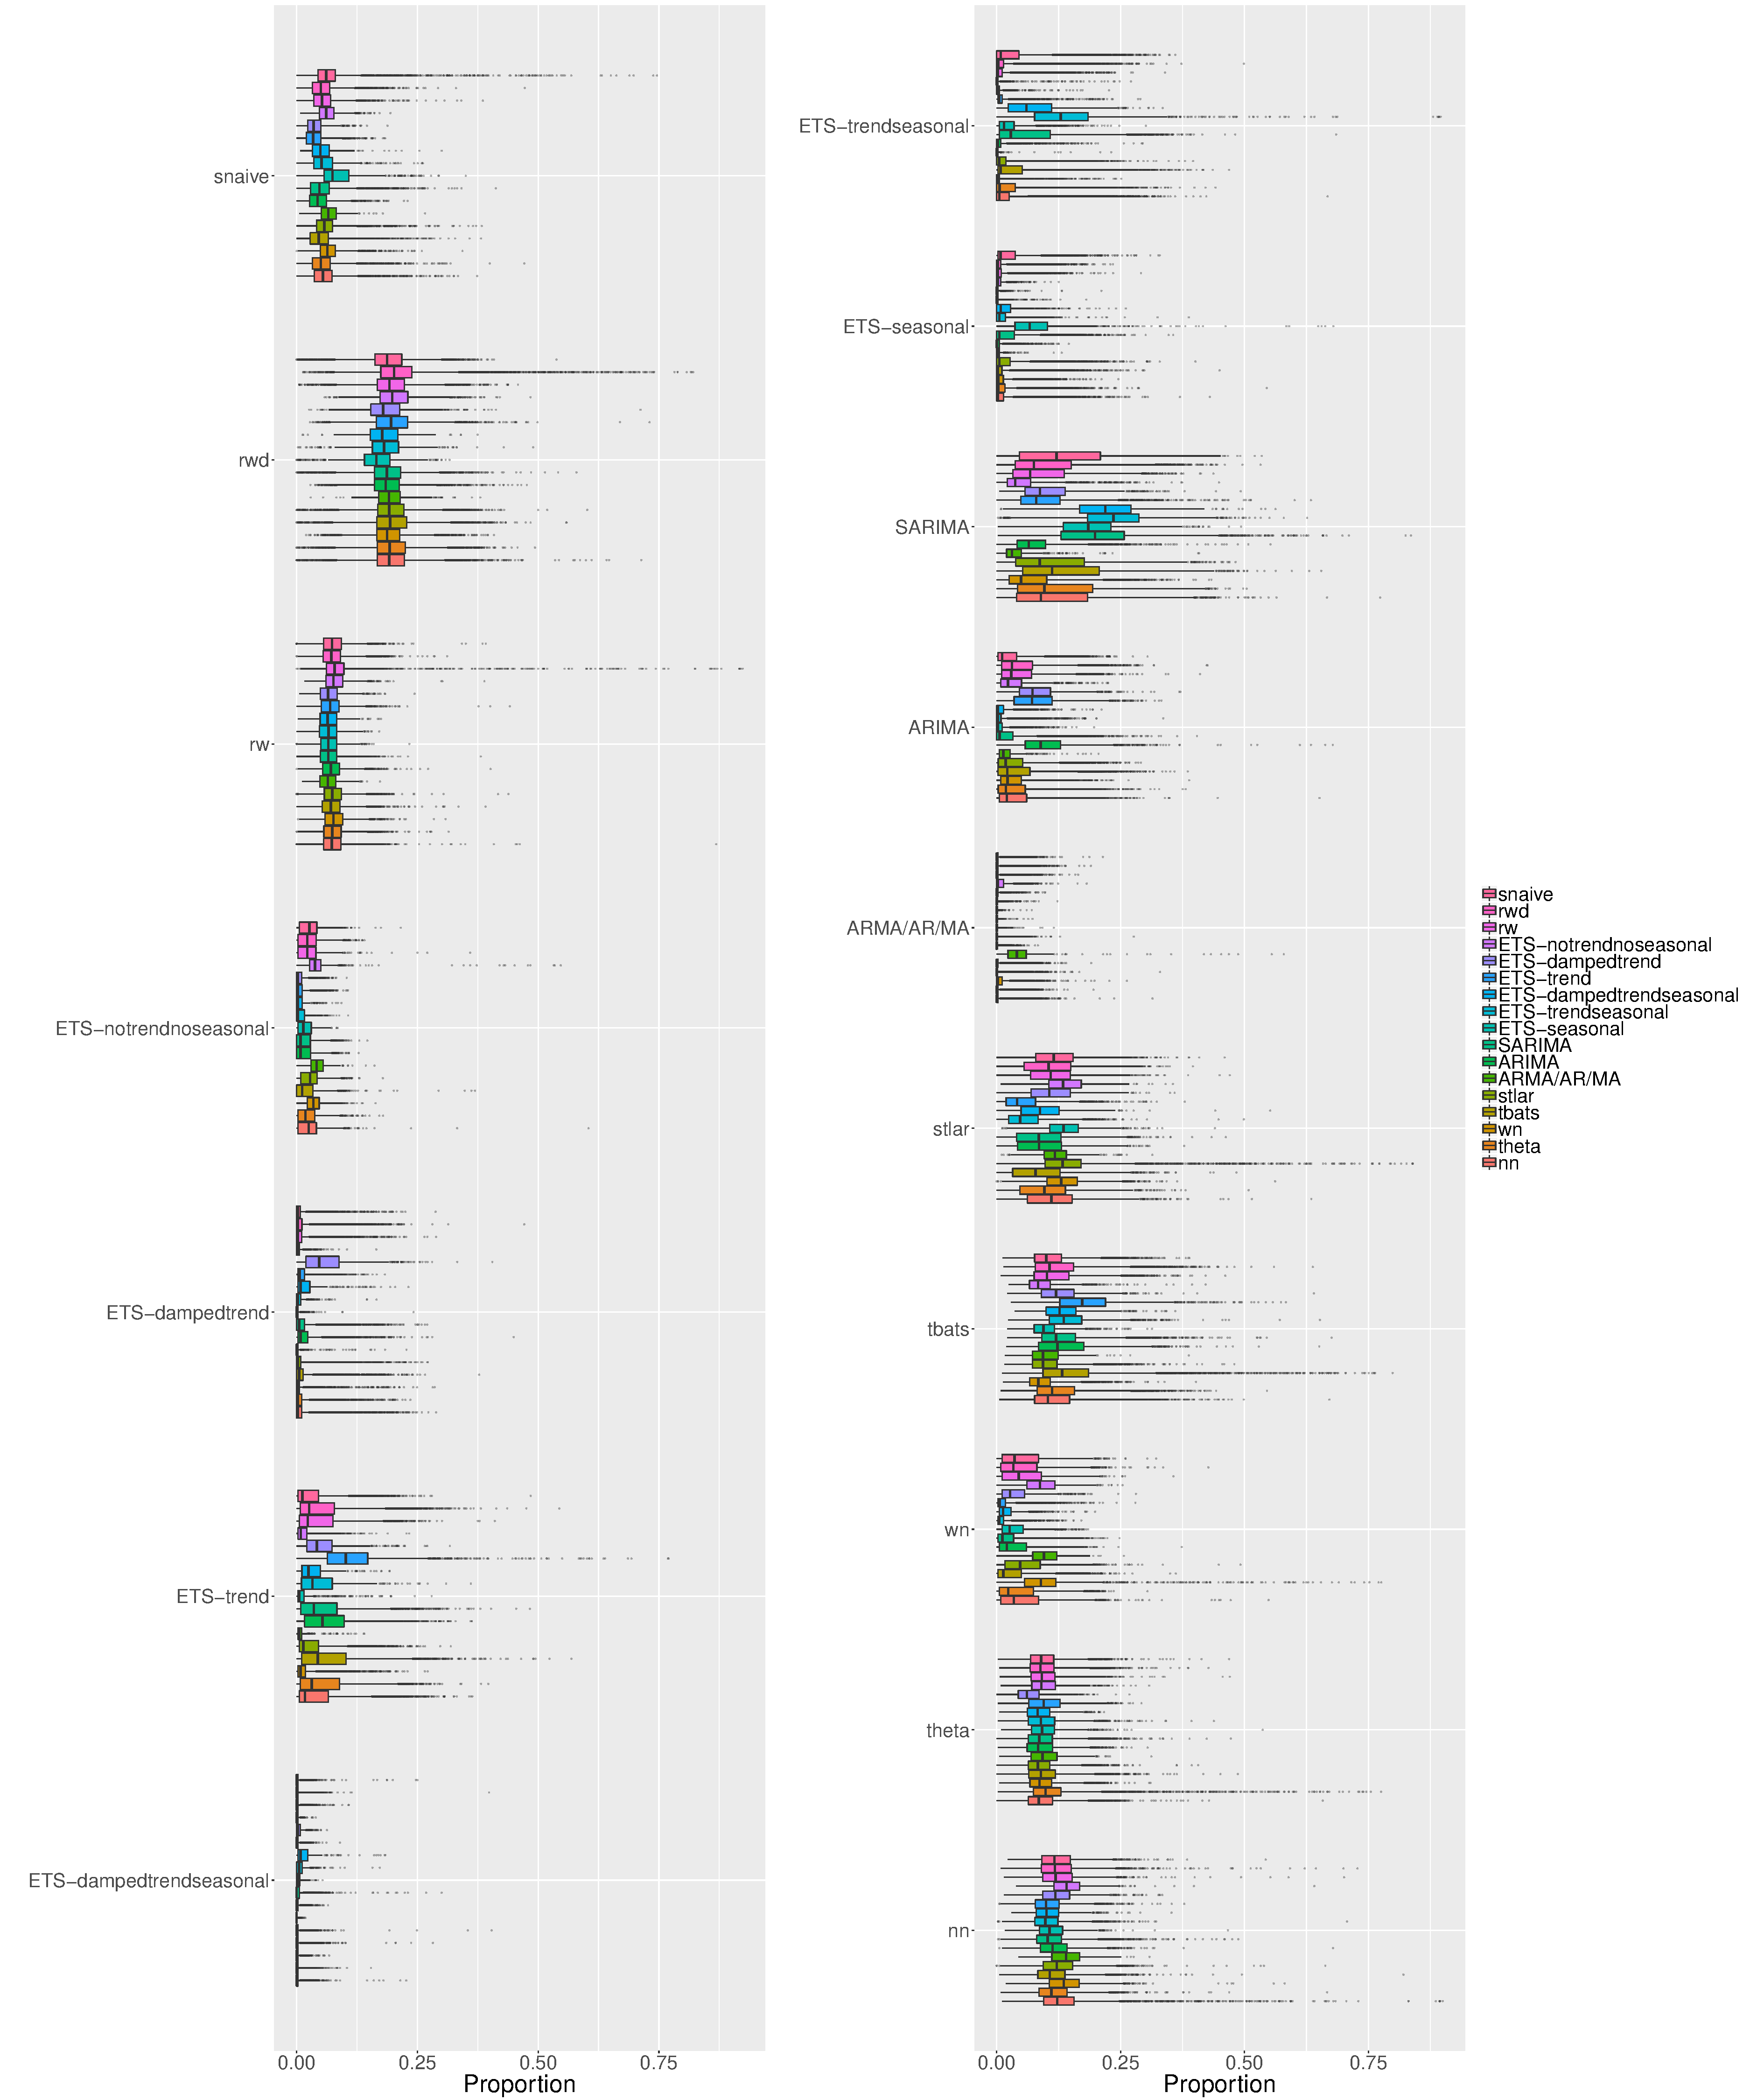
\includegraphics{figures/oobquarterlymonthly1-1.pdf}
\caption{\label{fig:oobquarterlymonthly1}Distribution of proportion of times
each quarterly time series was assigned to each class based on OOB
sample. Each row represent the predicted class label and colours of
boxplots corresponds to class label of ``best'' forecasting method.
X-axis denotes the proportion of times the time series was predicted
into each class.}
\end{figure}

\clearpage

\begin{figure}
\centering
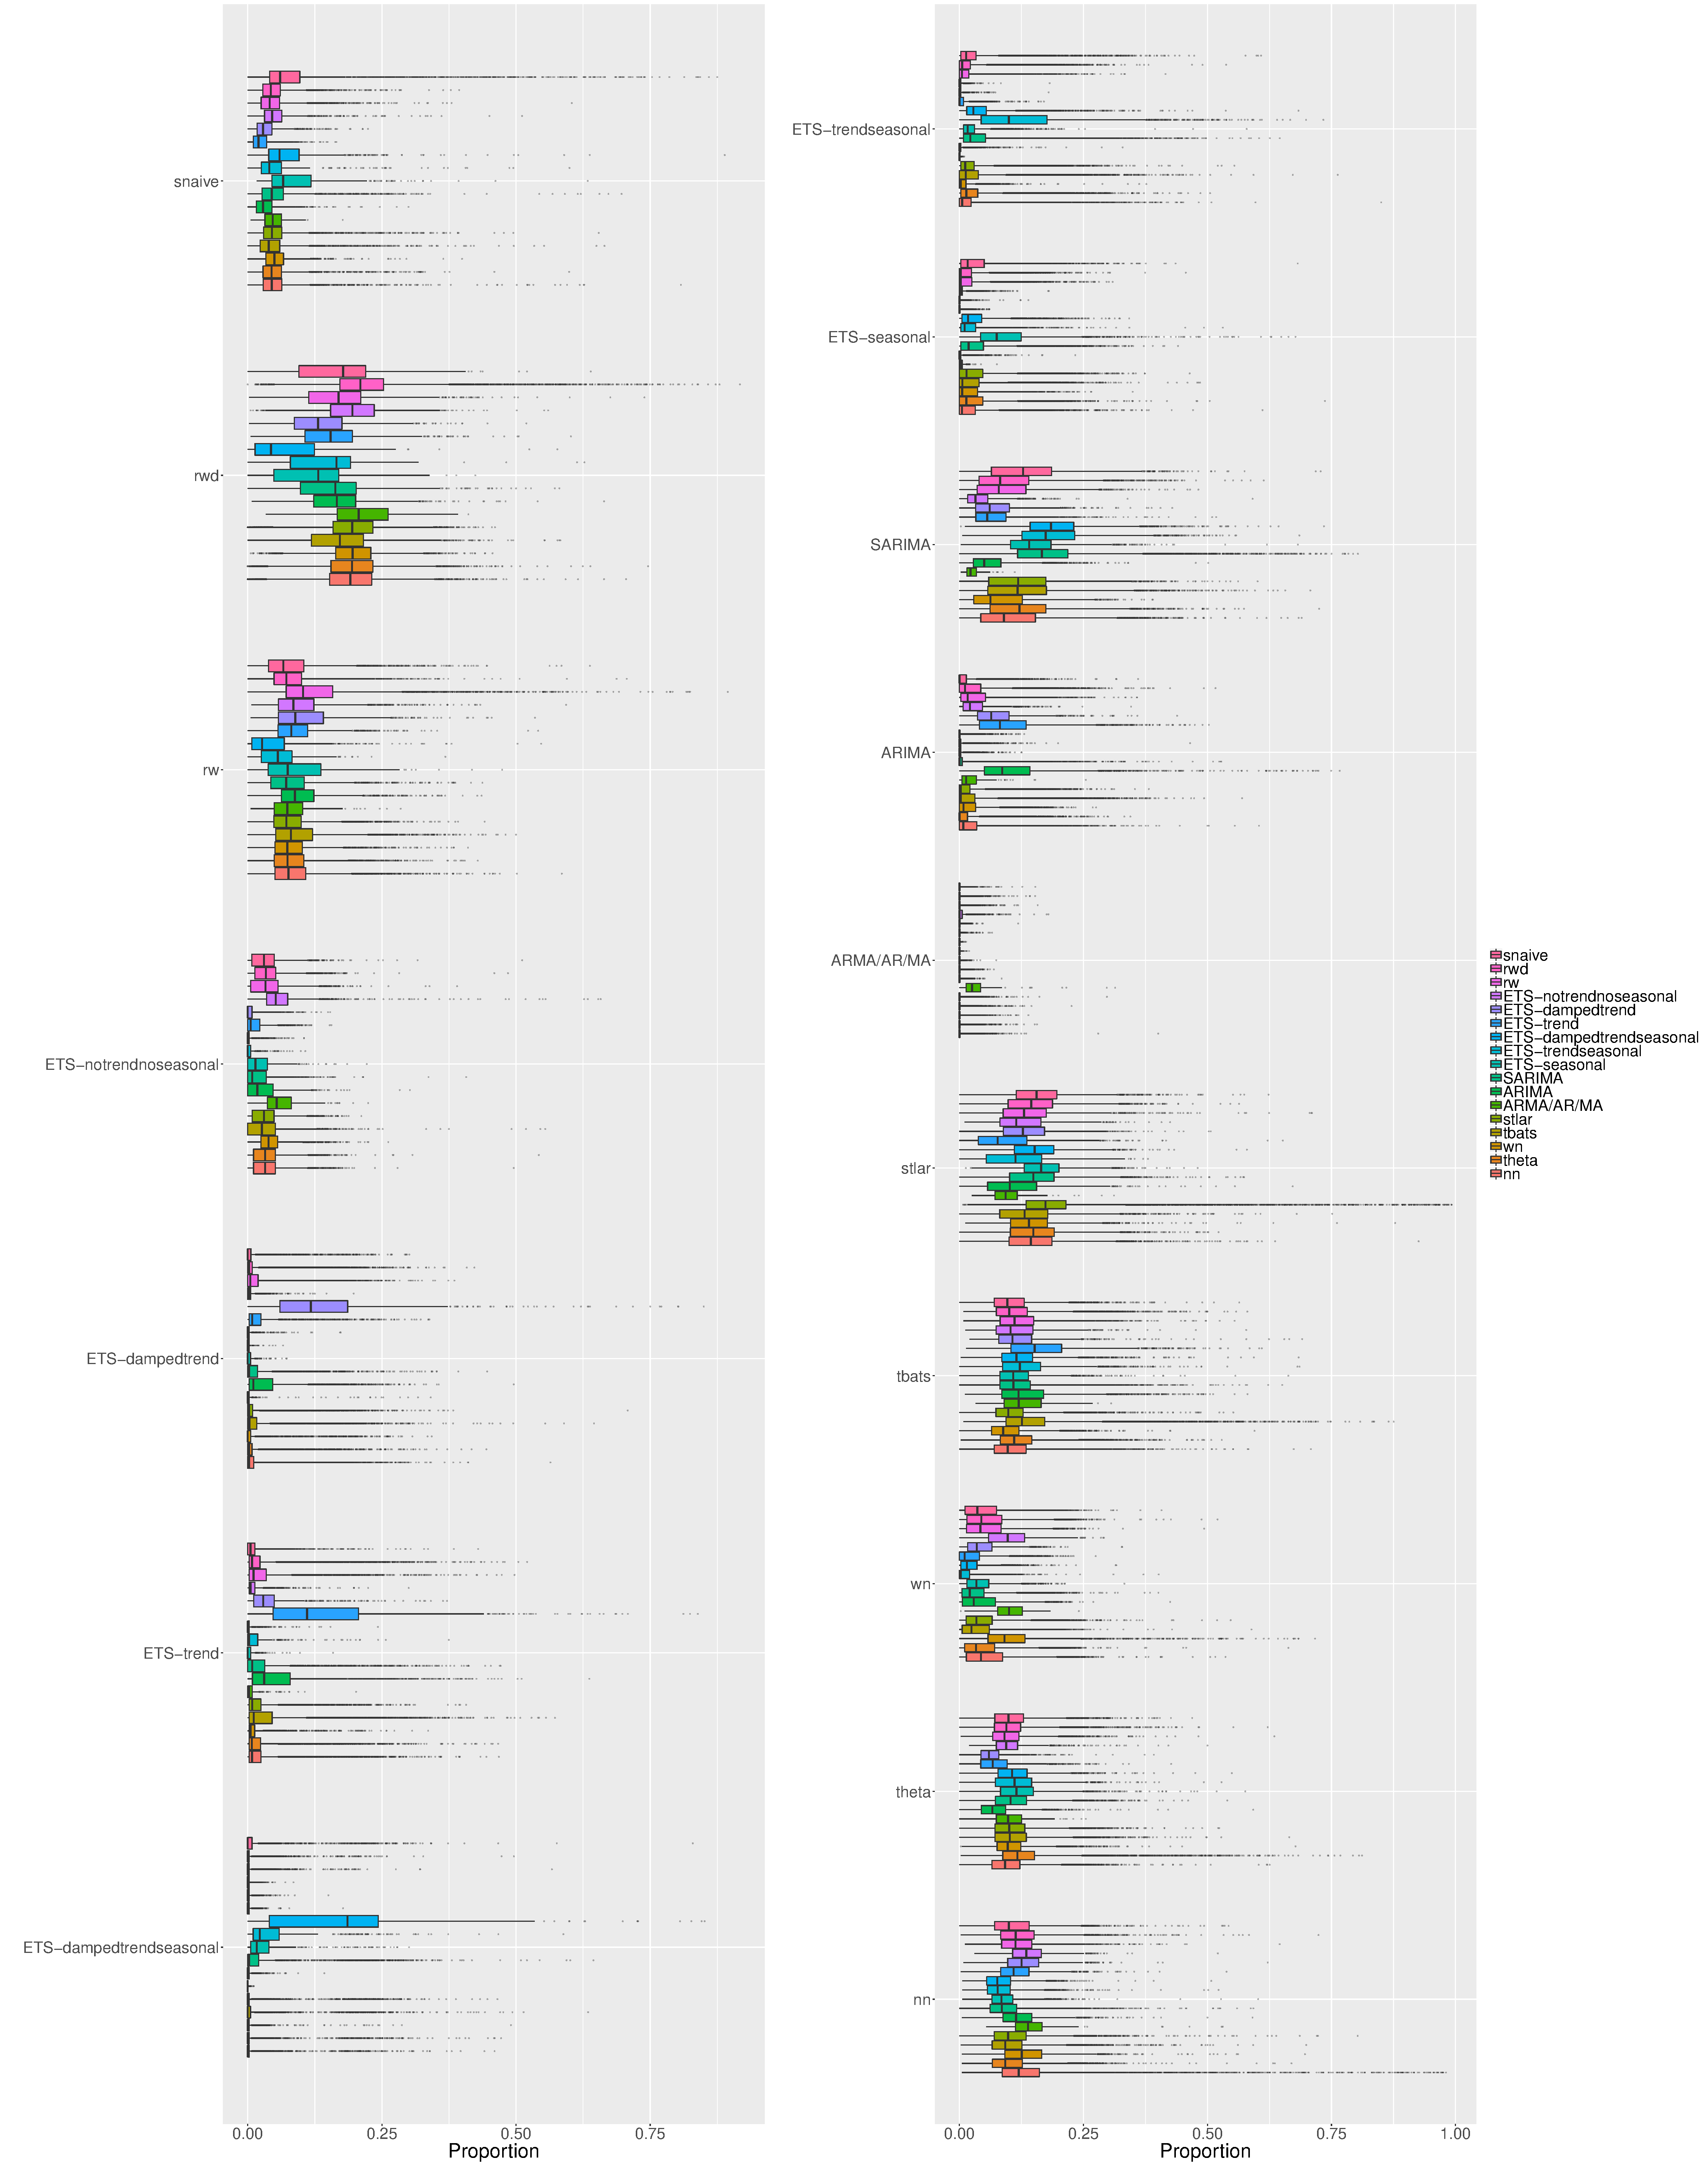
\includegraphics{figures/oobquarterlymonthly2-1.pdf}
\caption{\label{fig:oobquarterlymonthly2} Distribution of proportion of
times each monthly time series was assigned to each class based on OOB
sample. Each row represent the predicted class label and colours of
boxplots corresponds to class label of ``best'' forecasting method.
X-axis denotes the proportion of times the time series was predicted
into each class.}
\end{figure}

\clearpage

\begin{figure}[h]

{\centering \includegraphics{figures/viquarterly-1} 

}

\caption{Feature importance plot for quarterly data. Permutation-based VI measure and mean decrease in Gini coefficients are used to evaluate overall feature importance. Class-specific feature importance is evaluated based on the three measures: permutation-based VI, PD-based VI measure, and ICE-based VI measure. Longer bars indicate more important features. Top 5 features are highlighted in red.}\label{fig:viquarterly}
\end{figure}

\begin{figure}[h]

{\centering \includegraphics{figures/vimonthly-1} 

}

\caption{Feature importance plot for monthly data. Permutation-based VI measure and mean decrease in Gini coefficients are used to evaluate overall feature importance. Class-specific feature importance is evaluated based on the three measures: permutation-based VI, PD-based VI measure, and ICE-based VI measure. Longer bars indicate more important features. Top 5 features are highlighted in red.}\label{fig:vimonthly}
\end{figure}

\newpage

\begin{figure}
\centering
\includegraphics{figures/pdpquarterly1-1.png}
\caption{\label{fig:pdpquarterly1}Partial dependence plots for the top-three
features get selected most within each class inside quarterly and
monthly FFORMS frameworks. Additionaly, N is included to observe the
effects stated in the liteature. The shading shows the 95\% confidence
interval. Y-axis denotes the probability of belonging to corresponding
class. Red coulour is for PDP drawn based on quarterly data and blue
colour is for the PDP drawn based on monthly data.}
\end{figure}

\newpage

\begin{figure}
\centering
\includegraphics{figures/pdpquarterly2-1.png}
\caption{\label{fig:pdpquarterly2}Partial dependence plots for the top-three
features get selected most within each class inside quarterly and
monthly FFORMS frameworks. Additionaly, N is included to observe the
effects stated in the liteature. The shading shows the 95\% confidence
interval. Y-axis denotes the probability of belonging to corresponding
class. Red coulour is for PDP drawn based on quarterly data and blue
colour is for the PDP drawn based on monthly data.(Continue from Figure
9)}
\end{figure}

\newpage

\begin{figure}
\centering
\includegraphics{figures/friedmanQ-1.pdf}
\caption{\label{fig:friedmanQ}Heat maps of relative strength of all possible
pairwise interactions calclated based on Friedman's H-statistic for
quarterly data.}
\end{figure}

\newpage

\begin{figure}
\centering
\includegraphics{figures/friedmanM-1.pdf}
\caption{\label{fig:friedmanM}Heat maps of relative strength of all possible
pairwise interactions calclated based on Friedman's H-statistic for
monthly data.}
\end{figure}

\subsection{Weekly}\label{weekly}

\autoref{fig:oobweekly} shows the proportion of times each time series
was classified to each class. Unlike, yearly, quarterly and monthly data
theta method have a low chance of being selected to forecast weekly
data. The random walk with drift, tbats models and theta have higher
chance of being selected. Except ARMA/AR/MA class the distribution
corresponds to the true class label dominates others. ARMA/AR/MA class
shows some unusual behaviour within some categories due to class
imbalance ratio, ARMA/AR/MA class contains fewer number of observations
in the training set.

\begin{figure}
\centering
\includegraphics{figures/oobweekly-1.png}
\caption{\label{fig:oobweekly}Distribution of proportion of times each
weekly time series was assigned to each class based on OOB sample. Each
row represent the predicted class label and colours of boxplots
corresponds to class label of ``best'' forecasting method. X-axis
denotes the proportion of times the time series was predicted into each
class.}
\end{figure}

\clearpage

According to the results of \autoref{fig:viweekly} spikiness, linearity,
trend, strength of seasonality, stability and lumpiness has been
assigned a high importance. This is similar to the results of yearly,
quarterly and monthly data. The length of series has been selected among
top 5 by mstlets, tbats, theta and neural network models. According to
the results of \autoref{fig:weeklypdp} for mstlets models probability of
being selected increases as the linearity increases while the opposite
relationship was observed at SARIMA models. It is surprising to observe
that for mstlets models probability of being selected decreases as
seasonality increases. This could be due to the interaction effect of
seasonality with others. According to \autoref{fig:friedmanHW}, for
weekly data, the number of pairs showing a particular degree of
interaction strength is relatively low compared to other yearly,
quarterly and monthly data. In tbats class, trend, linearity, spikiness,
seasonality and first autocorrelation coefficient of the seasonally
differenced series interact heavily with other features.

\begin{figure}[h]

{\centering \includegraphics{figures/viweekly-1} 

}

\caption{Feature importance plot for weekly data. Permutation-based VI measure and mean decrease in Gini coefficient are used to evaluate overall feature impotance. Class-specific feature importance is evaluated based on the three measures: permutation-based VI, PD-based VI measure, and ICE-based VI measure. Longer bars indicate more important features. Top 5 features are highlighted in red.}\label{fig:viweekly}
\end{figure}

\newpage

\begin{figure}
\centering
\includegraphics{figures/weeklypdp-1.png}
\caption{\label{fig:weeklypdp}Partial dependence plots for the top ranked
features from variable importance measures (weekly series). The shading
shows the 95\% confidence intervals. Y-axis denotes the probability of
belong to corresponding class.}
\end{figure}

\newpage

\begin{figure}
\centering
\includegraphics{figures/friedmanHW-1.pdf}
\caption{\label{fig:friedmanHW}Heat maps of relative strength of all
possible pairwise interactions calclated based on Friedman's H-statistic
for weekly data.}
\end{figure}

\newpage

\subsection{Daily and Hourly data}\label{daily-and-hourly-data}

According to \autoref{fig:oobdailyhourly} the distributions corresponds
to observations that have been correctly classified dominated the top
for daily data. However, within daily series there are few observations
that have been incorrectly classified to tbats class with very high
probabilities. In general, neural network models have higher chance of
getting selected for daily time series. Overall, for hourly series
random walk with drift models, tbats and neural network models have high
chance of getting selected. Furthermore, it is important to note that
all hourly series have been assigned non-zero probability of getting
selected to neural network class. Variable importance graph for daily
and hourly data are shown in \autoref{fig:vidaily} and
\autoref{fig:vihourly} respectively. The most important features for
determining suitable forecast-models for daily time series are, strength
of seasonality corresponds to the weekly seasonality (7, measured by
seasonal\_strength1), stability, trend, lumpiness and linearity.
Strength of seasonality corresponds to the annual seasonality (365.25,
measured by seasonal\_strength2) is appeared to be important in
determining the selection of theta models. Furthermore, length of the
series is important in determining random walk, random walk with drift,
mstlarima, mstlets, stlar, theta and nn classes. \autoref{fig:dailypdp}
shows the partial dependency plots of the top 3 features from the FFORMS
framework. According to the results of \autoref{fig:dailypdp} shorter
series tends to select random walk with drift models while probability
of selecting snaive, mstlarima and mstlets models increases as the
length of series increases. Neural network models shows a non-monotonic
relationship with length of the series (N). The theta models tends to be
selected for series with high annual seasonality but very low weekly
seasonality. According to \autoref{fig:vihourly}, strength of daily
seasonality (period=24, measured by seasonal\_strength1) appear to be
more important than than the strength of weekly seasonality (period=168,
measured by seasonal\_strength2). Furthermore, entropy, linearity, sum
of squares of first 5 coefficients of PACF, curvature, trend, spikiness
and stability were found to be the most important features in
determining best forecasting method for hourly time series. Only snaive
category ranked N among top 5 for hourly time series. The strength of
seasonality corresponds to weekly seasonality also seems to be one of
the most important feature for the classes snaive, random walk,
mstlarima, and tbats. According to \autoref{fig:hourlypdp} probability
of selecting random walk, random walk with drift, theta model and white
noise process decreased with higher strength of daily
(seasonal\_strength1) seasonality, while the opposite relationship hold
for other classes. On the other hand, probability of selecting random
walk model increased with the increase in strength of weekly
seasonality.

\begin{figure}
\centering
\includegraphics{figures/oobdailyhourly-1.png}
\caption{\label{fig:oobdailyhourly}Distribution of proportion of times each
daily time series was assigned to each class in the forest. Each row
represent the predicted class label and colour of boxplots corresponds
to true class label. There are ten rows in the plot corresponds to each
predicted class represented by Y-axis. X-axis denotes the proportion of
times a time series is classified in each class. On each row,
distribution of correctly classified class dominated the top, indicating
a fairly good classification of the model fitted.}
\end{figure}

\newpage

\begin{figure}[h]

{\centering \includegraphics{figures/vidaily-1} 

}

\caption{Feature importance plot for daily data. Permutation-based VI measure and mean decrease in Gini coefficients are used to evaluate overall feature importance. Class-specific feature importance is evaluated based on the three measures: permutation-based VI, PD-based VI measure, and ICE-based VI measure. Longer bars indicate more important features. Top 5 features are highlighted in red.}\label{fig:vidaily}
\end{figure}

\begin{figure}
\centering
\includegraphics{figures/vihourly-1.png}
\caption{\label{fig:vihourly}Feature importance plot hourly series.
Permutation-based VI measure and mean decrease in Gini coefficients are
used to evaluate overall feature importance. Class-specific featue
importance is evaluated based on the three measures: permutation-based
VI, PD-based VI measure, and ICE-based VI measure. Longer bars indicate
more important features. Top 5 features are highlighted in red.}
\end{figure}

\newpage

\begin{figure}
\centering
\includegraphics{figures/dailypdp-1.png}
\caption{\label{fig:dailypdp}Partial dependence plots for the top ranked
features from variable importance measures(daily series). The shading
shows the 95\% confidence intervals. Y-axis denotes the probability of
belong to corresponding class. (seasonal\_strength1 denotes weekly
seasonality and seasonal\_strength2 for annual seasonality).}
\end{figure}

\newpage

\begin{figure}
\centering
\includegraphics{figures/hourlypdp-1.png}
\caption{\label{fig:hourlypdp}Partial dependence plots for the top ranked
features from variable importance measures(hourly series). The shading
shows the 95\% confidence intervals. Y-axis denotes the probability of
belong to corresponding class.(seasonal\_strength1 denotes daily
seasonality and seasonal\_strength2 for weekly seasonality)}
\end{figure}

\newpage

\begin{figure}
\centering
\includegraphics{figures/friedmandailyhourly-1.pdf}
\caption{\label{fig:friedmandailyhourly}Heat maps of relative strength of
all possible pairwise interactions calclated based on Friedman's
H-statistic for daily and hourly data.}
\end{figure}

\newpage

\subsection{Local Interpretable Model-agnostic
Explanations}\label{local-interpretable-model-agnostic-explanations}

\autoref{fig:yearlylime2}-\autoref{fig:hourlylime2} show the feature
contribution for the instances highlighted in the PCA-space for yearly,
quarterly and hourly series respectively. Different types of time series
under different frequency categories that are classified with high
probability are highlighted. The low linearity, with a trend value of
less than 0.616, low values for Phillip-Perron test-statistic, Hurst
exponent, autocorrelation coefficients of the time series and spikiness
of the series causes the FFORMS framework to classify the first series
with ARMA/AR/MA. On the other hand, LIME indicated the low value of
first autocorrelation coefficients of the original series and the
residual series of linear regression model contradicts to this decision.
It is interesting to note that even though 2, 4 and 5 series located
close proximity to each other in the PCA space their varying degree of
trend, spikiness, first autocorrelation coefficient of the difference
series, entropy, led them to classify as ETS-trend, neural-network and
random walk respectively. From \autoref{fig:quarterlylime2} we can see
how the different variation in strength of seasonality influence the
FFORMS framework to select different types of forecast-models. For
example, SARIMA models was selected when the seasonality vary between
0.579 and 0.787 (case 1), ETS-seasonal models is selected when the
strength of seasonality is greater than 0.787 (case 4), random walk with
drift when the seasonality with lower than 0.579 (case 2) and for the
highly trended and seasonal series (strength of seasonality
\textgreater{} 0.895) ETS model with a trend and seasonal component is
selected (case 3). According to \autoref{fig:hourlylime2} FFORMS
framework selected \texttt{mstlarima} for the fourth series due to
strong multiple seasonality corresponds to weekly (measured my
seasonal\_strength2) and daily (measured my seasonal\_strength1). From
the global explanations we observed that strength of daily seasonality
has been assigned a very high importance. In addition to that, according
to the LIME explanation strong weekly seasonality present in the data
supports the decision of selecting mstlarima models. For the second
hourly series the strength of seasonality corresponds to both weekly and
daily supports the decision of selecting tbats models. This is true as
the TBATS models are capable of handling series with multiple complex
seasonalities. Further, lime explanation of hourly series suggests high
value of trend, low value of spikiness contradicts to the decision of
selecting neural network model to the third hourly series but ACF-based
features related to seasonal lags, high length, high linearity (value
increases as time index increases) and long term positive
autocorrelation (Hurst exponent \textgreater{} 0.99) support the FFORMS
decision in selecting neural network model. From LIME approach we can
gain insight into the local neighbourhood characteristics which lead to
the choice of a particular neighbourhood over alternative destinations.

\clearpage

\begin{figure}[h]

{\centering \includegraphics{figures/yearlylime-1} 

}

\end{figure}

\begin{figure}[h]

{\centering \includegraphics{figures/yearlylime2-1} 

}

\caption{Panel A: Distribution of yearly time series in the PCA space. Panel B: Time series corresponds to the highlighted points in the PCA space. Panel C: Local interpretable Model-agnostic explanations for six selected yearly time series. Features denoted with green colour are supporting features for an outcome label and length of the bar is proportional to the weight of a feature.}\label{fig:yearlylime2}
\end{figure}

\clearpage

\begin{figure}[h]

{\centering \includegraphics{figures/quarterlylime-1} 

}

\end{figure}

\begin{figure}[h]

{\centering \includegraphics{figures/quarterlylime2-1} 

}

\caption{Panel A: Distribution of quarterly time series in the PCA space. Panel B: Time series corresponds to the highlighted points in the PCA space. Panel C:Local interpretable Model-agnostic explanations for four selected quaterly time series. Features denoted with green colour are supporting features for an outcome label and length of the bar is proportional to the weight of a feature.}\label{fig:quarterlylime2}
\end{figure}

\clearpage

\begin{figure}[h]

{\centering \includegraphics{figures/hourlylime-1} 

}

\end{figure}

\begin{figure}[h]

{\centering \includegraphics{figures/hourlylime2-1} 

}

\caption{Panel A: Distribution of hourly time series in the PCA space. Panel B: Time series corresponds to the highlighted points in the PCA space. Panel C:Local interpretable Model-agnostic explanations for four selected hourly time series. Features denoted with green colour are supporting features for an outcome label and length of the bar is proportional to the weight of a feature.}\label{fig:hourlylime2}
\end{figure}

\clearpage

\section{Discussion and Conclusions}\label{conclusions}

Forecast model selection is both time and computer cost intensive
process. Consequently, the application of machine-learning approaches to
predict suitable forecasting model from large number of potentially
relevant time series features is a topic growing popularity in the field
of time series forecasting. Recently we introduced a computationally
efficient framework for individual forecast models selection based on
the features computed from the time series. We called this framework
FFORMS: Feature-based FORecast Model-Selection. The M4-competition
submission based on FFORMS framework was placed eighth under prediction
interval category. In this paper we used model-agnostic machine learning
interpretability tools to explore what was happening under the hood of
FFORMS framework and to gain an understanding of what features led to
the choices of FFORMS framework. On the other hand explaining
predictions is an important aspect in getting humans trust and use the
proposed framework effectively, if the explanations are faithful and
intelligible. Humans usually have prior knowledge about the application
domain, which they can use to accept (trust) or reject prediction if
they understand the reasons behind it.

We explored the role of features in two different perspectives: i)
individual effect of feature, and ii) interaction effect of features.
Overall, the features strength of trend, strength of seasonality,
linearity, spikiness and curvature among the top 10 within each
frequency category. \textcite{lemke2010meta} also pointed out features
related to nonstationarity and seasonality of a series are important
factors for choosing a forecasting method. Features that frequently
appear can be considered as more relevant than those that tend to appear
less frequently. Partial dependency plots are used to visualize the
learned relationship between features and the model predictions. The
displayed relationships confirm to domain knowledge expectations.
However, since several number of features are used to build the
framework with comparable contributions, and thus, all individual
contributions are small. According to the results of daily and hourly
data we also observed neural network modelling model was appropriate for
forecasting high frequency data. In response to the results of the
M3-competition this has been pointed out by many commentators
\autocite{makridakis2000m3}. Further, our results show that the
performance of various methods depends upon the length of the time
series. Short time series tends to select simple methods such as random
walk models, snaive, etc. ETS models with both trend and seasonal
components, SARIMA models, mstl models tend to provide accurate
forecasts with longer time series as these are more parameterized
models.

As FFORMS framework is developed on top of random forest algorithm takes
into account every possible interactions. We used Friedman's H-statistic
to identify most important two-way interactions. It was apparent from
the heat matrices of Friedman's H-Statistic presented that a substantial
interaction effect exist between the features. The strength trend showed
less interactivity in yearly series data,reflecting that these features
are more important on their own. The features involve in interaction and
their strength of interaction effect differ across the different
frequency categories (yearly, quarterly, monthly, weekly, daily and
hourly) as well as forecast-models (random walk, ETS models, etc.).
However, it is interesting to note that in each frequency category all
or subset of ACF/PACF-based features interact each other. This confirm
that information regarding correlation structure of the time series is
an essential information for the choice of model selection.
\autoref{fig:ytwopdp} - \autoref{fig:htwopdp} show partial dependency
plot for most frequently appeared interacting feature combination in
each of the frequency categories. According to figures
\autoref{fig:ytwopdp} - \autoref{fig:htwopdp} the unique pattern of
interactivity exist within each class are useful for separating one from
another.

Exploration of conditions learnt by the FFORMS framework also support
practitioners to make a good educated guess on suitable forecast-model
for a given problem. Further the results of this study is useful in
identifying new ways to improve forecasting accuracy by capturing
different features of time series.

\newpage

\section*{Appendix}\label{appendix}
\addcontentsline{toc}{section}{Appendix}

\begin{figure}
\centering
\includegraphics{figures/ytwopdp-1.png}
\caption{\label{fig:ytwopdp}Partial dependece plot of model selection
probability and the interaction of stability and lumpiness for yearly
data. As seen in Figure 1 ETS-dampedtrend and ARMA/AR/MA has low
probability of selecting. Hence less diversity is observed in the
corresponding two-way interaction plots. ETS-notrendnoseasonal, ARIMA
and theta classes show similar pattern of interactivity.}
\end{figure}

\begin{figure}
\centering
\includegraphics{figures/qtwopdp-1.png}
\caption{\label{fig:qtwopdp}Partial dependence plot of model selection
probability and the interaction of stability and diff1y\_acf5 for
quarterly data. The classes snaive, random walk and random walk with
drift show similar pattern of interactivity while the white noise class
hold the opposite pattern of interactivity. ETS-dampedtrend and
ARMA/AR/MA classes low probability of selecting for forecasting
quarterly time series hennce low variation in the interaction pattern
can be observed.}
\end{figure}

\begin{figure}
\centering
\includegraphics{figures/mtwopdp-1.png}
\caption{\label{fig:mtwopdp}Partial dependence plot of model selection
probability and the interaction of sediff\_seacf1 and sediff\_acf5 for
monthly data. Interaction between sediff\_seacf1 and sediff\_acf5 do not
influence the choice of ETS-dampedtrend and ARMA/AR/MA.}
\end{figure}

\begin{figure}
\centering
\includegraphics{figures/wtwopdp-1.png}
\caption{\label{fig:wtwopdp}Partial dependence plot of model selection
probability and the interaction of trend and entropy for weekly data.
Unique pattern of interactivity exist within each class. ARIMA and white
noise class show opposite direction of interactivity between trend and
entropy.}
\end{figure}

\begin{figure}
\centering
\includegraphics{figures/dtwopdp-1.png}
\caption{\label{fig:dtwopdp}Partial dependence plot of model selection
probability and the interaction of sediff\_acf5 and seasonal\_strength2
for daily data. Within each class unique pattern of interaction pattern
exist between sediff\_acf5 and seasonal\_strength2.}
\end{figure}

\begin{figure}
\centering
\includegraphics{figures/htwopdp-1.png}
\caption{\label{fig:htwopdp}Partial dependence plot of model selection
probability and the interaction of sediff\_seacf1 and linearity for
hourly data. Random walk and random walk with drift class show opposite
pattern of interactivity between sediff\_seacf1 and linearity.}
\end{figure}

\newpage

\printbibliography[title=References]

\end{document}
